\documentclass[a4j]{ujarticle}
\usepackage[dvipdfmx]{graphicx}
\usepackage{url}
\usepackage{bbding}
\usepackage{lscape}
\usepackage[subrefformat=parens]{subcaption}
\usepackage{bm}
\usepackage{amsmath}

\title{ミーティング資料}
\author{安達智哉\\to-adachi@ist.osaka-u.ac.jp}
\date{2019年8月9日}

\begin{document}
\maketitle


\section{はじめに}
  \label{sec:abs}
MMEおよびSGW、PGWなどのEPCノードは、主なリソースとしてCPUとメモリを持っている。
CPUは、アタッチやデタッチなどのシグナリング処理を実行するために必要とされるリソースである。
一方メモリは、ベアラなどのセッション情報を保持するために必要とされるリソースである。
これらのリソースは、モバイルネットワークにおける通信を可能にするために必須であるため、ネットワーク事業者は、どちらのリソースも枯渇することがないように、CPUとメモリをバランスよく割り当てる必要がある。

その一方で、近年はM2M/IoT端末の急激な増加が注目されている。
M2M/IoT端末は通信特性において従来の端末(携帯電話やスマートフォンなどのユーザ端末)とは大きく異なり、データの送信に周期性や間欠性を持つという特徴がある。
そのため、データの送信ごとにidle状態とconnected状態を遷移することが予想される。
その結果、端末のネットワーク接続やデータ送信に必要なシグナリングに関する通信や処理を行う、制御プレーンの輻輳が悪化すると考えられる。
また、M2M/IoT端末は消費電力を抑えることが必要とされている。
このような問題に対し、RRC Connected Inactiveと呼ばれるM2M/IoT端末の新たなのステートを導入することによって、消費電力およびシグナリングの削減を目標とする研究が行われている。
% RRC Suspendedとは、M2M/IoT端末のコンテキストが端末及びネットワークに保存されている状態であり、
RRC Connected Inactiveとは、M2M/IoT端末のコンテキストが端末及びネットワークに保存され、RAN-CN間の接続がアクティブ状態で維持されている状態である。
Connected Inactive状態においては、一部の情報が保持されているため、connected状態へ遷移する際に発生するシグナリングは、idle状態とconnected状態を遷移することによって発生するシグナリングよりも小さくなることが予想される。さらに、シグナリングの削減に伴い、端末の消費電力削減も期待できる。
実際、文献\cite{RRCStateHandlingfor5G}および\cite{ANovelStateModelfor5GRadioAccessNetworks}においては、RRC Connected Inactiveを導入することにより、シグナリングオーバヘッドの削減および消費電力の削減が可能であることを示している。

上述のRRC Connected InactiveをM2M/IoT端末に適応することは、CPUやメモリなどのサーバリソースの効率的な割り当てを難しくすると考えられる。
なぜなら、RRC Connected Inactive	はその特性から、端末がデータを送信していないタイミングにおいてもその端末情報をネットワークに保持するため、コアネットワークノードのメモリに対してこれまで以上の大きな負荷を発生させるためである。
また、M2M/IoT端末の接続台数の予測が難しいこともリソースの割り当てを難しくする一因である。
M2M/IoT端末は、スマートフォンのようなユーザ端末とは異なり、家電や自動車、電気メーター、センサなど様々な場所、様々な用途で使用される可能性があり、端末の台数およびその分布を予測することは困難であると考えられる。
さらには、それらの端末の送信タイミングを把握することも容易ではない。
このように、新たな状態の導入や、接続台数の予測が難しいIoT端末の普及により、今後のネットワーク事業者は、コアネットワークノードへのサーバリソースの割り当てがより難しくなると予想される。

上述のようなネットワーク(サーバリソース消費の予測が難しく、変動が激しいネットワーク)において、収容可能な端末の増加を目的とした既存研究には、スケールアウトの考え方を用いたものが多い。
これらの研究では主に稼働するサーバやインスタンスの数をリソースの需要に応じて変動させることにより、ネットワークの変動に対応している\cite{Scale-OutArchitectureforServiceOrderProcessingSystems}。
しかし、この方法では、本来必要とされているリソース量(需用量)よりも多くのリソースが供給される、オーバープロビジョニングが発生する問題がある。
なぜなら、これらの研究では、サーバやインスタンス一台あたりのリソース量は一定であることを前提にした研究が多く、細かい粒度でリソースを制御できないためである。
また、必要とされるCPUとメモリのリソース比があらかじめ分かっていることを前提とした研究が多く、必要とされるリソース比が未知の場合はリソースの効率的な利用ができないからである。
例えば、CPUのリソース不足を解消するためにケールアウトを行った場合、CPUリソースと同時にメモリリソースも増加する。
しかし、メモリは元々ボトルネックにはなっていないため、新たに追加されたメモリはオーバープロビジョニングされたことになる。
文献\cite{ACloudNativeSolutionforDynamicAutoScalingofMMEinLTE}では、IoT端末を収容しているMMEを単純にスケールアウトした場合、処理リソースやメモリリソースが不必要にプロビジョニングされる可能性があることを述べている。

% 現在のモバイルネットワークでは、EPCノードにおけるCPUとメモリのリソース消費の予測が難しような状況や変動が大きいような状況においても、どちらかがボトルネックにならずに、効率的にリソースを活用するアーキテクチャを考えることは重要である。
このような背景から、EPCノードにおけるCPUとメモリのリソース消費の予測が難しような状況や変動が大きいような状況においても、どちらかのリソースがボトルネックにならずに、効率的にリソースを活用するアーキテクチャを考えることは重要である。
実際、CPUとメモリのリソースを効率よく活用する研究は、データセンタなどの分野では行われている。
文献\cite{TechnoEconomicFrameworkforCloudInfrastructureACostStudyofResourceDisaggregation}では、server disaggregation の考えをデータセンタに適用し、CPUやメモリなどのリソースをモジュール化し、需要に合わせて自由に組み替えることを可能にすることにより、リソースの効率的な利用が可能であることを示している。
しかし、server disaggregation にはいくつかの課題がある。
まず、CPUとメモリのリソースを分離するためには、大きなコストがかかる点が挙げられる。
文献\cite{IntelsDisaggregatedServerRack}、\cite{EnhancedBackoffTimerSolutionforGTPCOverloadControl}では、CPUとメモリを分離するためには、両者を結ぶための新しい高帯域ネットワークが必要になると述べている。また、両者の物理的な距離が増加することによって発生する遅延も考慮する必要があるため、新たなメモリアーキテクチャの構築が必要であると述べている。
文献\cite{DisaggregatedandOpticallyInterconnectedMemoryWhenwillitbecosteffective}では、メモリを分離するためには、低遅延かつ高帯域のネットワーク接続が必要となるが、それを実装するためのコストは従来と比較して大幅に増加すると述べている。
実際、文献\cite{DisaggregatedServersDriveDataCenterEfficiencyandInnovation}では、Disaggregated Serverに基づくインテルのラックスケールアーキテクチャを示しているが、このモデルでもCPUとメモリの分離はできていない。
課題の2つ目として、短いタイムスケールでの制御が難しいという問題が挙げられる。
これは、そもそもserver disaggregationは短いタイムスケールでのリソース制御を目的とした技術ではないためである。
例えば、ストレージをモジュール化してサーバと分離する手法について述べられている文献\cite{UnderstandingRackScaleDisaggregatedStorage}では、時間スケールの細かいストレージ制御を行った場合、ストレージの再割り当て処理に伴うオーバーヘッドが大きくなると述べている。
また、頻繁にリソース構成を変化させることは、コスト面や消費電力の面でも不利である。

このように、server disaggregation を用いたリソース制御では、リソース制御に伴うオーバーヘッドの発生が避けては通れない課題となると予想される。
特に、モバイルネットワークのように、突発的なトラヒックの増加が発生し、数分以下のオーダでリソース量の制御を行う必要があるネットワークにおいては細かいタイムスケールでの効率的なリソース制御が求められる。

そこで、本研究ではモバイルネットワークに特化した、柔軟かつ効率的な、EPCノードにおけるCPUとメモリ間の負荷のオフロード方法を考案する。
具体的には、ネットワークの負荷に合わせて、UEの状態を制御することにより、メモリおよびCPUに与える負荷のバランスを変化させる。
UEの状態の制御は、UEが最後にデータを送信したあと、Connected Inactive状態からIdle状態に遷移するまでの時間を設定することで実現する。
この方法により、CPUが過負荷である場合は、UEが最後にデータを送信したあと、Connected Inactive状態からIdle状態に遷移するまでの時間を長く設定することにより、メモリの負荷を増加させる代わりにCPUの負荷を削減することが可能である。
またその逆に、メモリが過負荷である場合は、この時間を短く設定することにより、CPUの負荷を増加させる代わりにメモリの負荷を削減できる。
この時間の再設定処理は、数分単位のオーダーで可能でありかつ、それに伴い発生するオーバーヘッドは、server disaggregation と比較して僅かである(注:提案手法のオーバーヘッドの大小に関する記述は、今後の研究結果によって修正します)。
また、既存のシグナリングアーキテクチャに変更を加えることが可能であれば、秒単位の時間スケールでの制御も可能であると考えられる。

しかし、提案手法には限界もある。
それは、対応可能なリソース需要に制限があることである。
なぜなら、提案手法では、限られたCPUおよびメモリのリソースを効率的に利用することは可能であるが、双方のリソースが過負荷になるようなリソース需要には対応できないからである。
特に長期的かつ大規模なリソース需要の変化に対しては、server disaggregation を用いたリソース制御の方が適している。
また、提案手法を用いなかった場合には常時Connected Inactive 状態であったUEが、提案手法を用いることによりIdle状態へと遷移する可能性があるため、データを送受信にかかる遅延時間が増加するなど、QoSの低下が発生する可能性がある。
しかし、電気メータや気温計のようなリアルタイム性を必要としないIoT端末であれば、これらのQoSの低下は無視できると考えられる。

そのため、提案手法とserver disaggregationやスケールアウト/スケールインを組み合わせることにより、より効果のあるリソース管理が可能であると考えられる。
例えば、長期的かつ大規模なリソース制御はserver disaggregationを用いて行う一方で、server disaggregation で対応できないような短いタイムスケールでのリソース制御は提案手法を用いて行う。
もしくは、リソース需要の大きな変動に対してはスケールアウト/スケールインを用いて対応した上で、細かなリソース需要の変化に対しては提案手法を用いて対応する。
上述ように、server disaggregationやスケールアウト/スケールインと提案手法組み合わせ、双方のデメリットを補うことで、モバイルネットワークのリソース制御をより良く実現できると考えられる。



\clearpage
\section{モバイルネットワークアーキテクチャ}
  \subsection{ネットワーク構成}
    図\ref{networkmodel}にモバイルネットワークを示す。モバイルネットワークは以下のノードから構成される。
    \begin{itemize}
      \item User Equipment (UE) :M2M/IoT端末。
      \item evolved NodeB (eNodeB) :UEと無線で通信を行い、MME及びS/PGWと制御通信を行う基地局。
      \item Mobility Management Entity (MME) :UEやユーザの認証、UEの移動管理及びパケットの経路設定の制御などを行い、EPC内におけるシグナリング処理の中核となるノード。
      \item Serving Gateway / Packet Data Network Gateway (S/PGW) :MMEからの制御メッセージに基づいて、LTE/EPCネットワークと外部のネットワーク(External IP Network) を接続するノード。UEがeNodeB間を移動した時のアンカーポイントとしても機能する。
      \item Home Subscliber Server (HSS) :ユーザごとの契約情報、認証用のキーデータ及びMMEのアドレスなどを管理するノード。
    \end{itemize}
    UEおよびeNodeBは複数台、その他のノードは1台づつ存在すると仮定する。
    \begin{figure}[htbp]
      \centering
      \includegraphics[width=0.7\hsize]{networkmodel.pdf}
      \caption{LTE/EPCネットワークモデル}
      \label{networkmodel}
    \end{figure}


  \subsection{UEのステート遷移}
    \subsubsection{従来のモバイルネットワークにおけるUEのステート遷移}
    従来のモバイルネットワークにおけるUEのステート遷移を図\ref{state_change_old}に示す。
    UEはデータ送信のタイミングでIdle状態からConnected状態へ遷移する。
    その後、一定時間データの送受信が発生しなければ、再びIdle状態へ遷移する。
    \begin{figure}[htbp]
      \centering
      \includegraphics[width=0.7\hsize]{state_change_old.pdf}
      \caption{従来のモバイルネットワークにおけるUEのステート遷移}
      \label{state_change_old}
    \end{figure}
    \subsubsection{Connected Inactiveを導入した場合におけるUEのステート遷移}
    Connected Inactiveを導入した場合におけるUEのステート遷移を図\ref{state_change_inactive}に示す。
    Idle状態のUEはデータ送信のタイミングで、Connected 状態へ遷移する。
    その後、一定時間データの送受信が発生しなければ、Connected Inactive状態へ遷移する。
    Connected Inactive状態のUEは、データ送信のタイミングで、Connected 状態へ遷移する。
    しかし、送信データサイズが小さい場合は、Connected状態への遷移を必要としない。
    また、Connected Inactive状態のUEは、例外的な処理が発生しない限り、Idle状態へは遷移しない。
    \begin{figure}[htbp]
      \centering
      \includegraphics[width=1.0\hsize]{state_change_inactive.pdf}
      \caption{Connected Inactiveを導入した場合におけるUEのステート遷移}
      \label{state_change_inactive}
    \end{figure}
    \subsubsection{Connected Inactiveにタイムアウト制御を適用した場合におけるUEのステート遷移(提案手法)}
    Connected Inactiveにタイムアウト制御を適用した場合におけるUEのステート遷移を図\ref{state_change_propose}に示す。
    Connected Inactive状態からIdle状態への状態遷移を追加したモデルである。
    \begin{figure}[htbp]
      \centering
      \includegraphics[width=1.0\hsize]{state_change_propose.pdf}
      \caption{Connected Inactiveにタイムアウト制御を適用した場合におけるUEのステート遷移}
      \label{state_change_propose}
    \end{figure}

\section{解析}
\label{seq:estimate}
EPCの負荷を求めるためには、EPCを構成する各ノードの負荷およびそれらを結ぶリンクの負荷などを全て考慮する必要がある。
しかし、今回対象とするUEはIoT端末であり、IoT端末はスマートフォンなどの従来の端末と比較すると送信データ量が非常に小さいという特徴があるため、データプレーンの負荷は十分小さいと仮定し、コントロールプレーンの負荷のみに着目する。
文献\cite{ACloudNativeSolutionforDynamicAutoScalingofMMEinLTE}では、コントロールプレーンの処理の中心的役割を担うノードはMMEであり、IoT端末を大量に収容した場合、MMEがEPCの中でのボトルネックになると述べている。
そのため今回の評価では、MMEに対して発生する負荷をコントロールプレーンの負荷として評価する。

MMEの負荷はシグナリングを処理することによって発生するCPU負荷と、UEのコンテキストを保持するこちによって発生するメモリ負荷に分けられる。
CPU負荷とメモリ負荷のバランスは、UEの状態遷移を制御することにより変えることが可能である。
具体的には、UEが最後にデータを送信したあと、Idle状態に遷移するまでの時間 ($T^{\rm i}$) を設定することで負荷のオフロードが可能である。
例えば、CPUが過負荷である場合は、$T^{\rm i}$を長く設定することにより、メモリの負荷が増加し、CPUの負荷が低下する。
またその逆に、メモリが過負荷である場合は、$T^{\rm i}$を短く設定することにより、CPUの負荷が増加し、メモリの負荷が低下する。

負荷を算出するにあたって以下のように条件を設定した。
\begin{itemize}
  \item UEごとに通信周期は固定であり、途中で変化することはない。
  \item データ送信にかかる時間はUEの通信周期と比べて十分小さいものとし、送信が失敗することはないと仮定する。
  \item UEの総数は有限かつ一定である。
  \item 算出する負荷は、UEの通信周期が理想的に分散しており、MMEに対して発生する負荷に関して時間的な変動がない場合の値である。現実的なモデルを考える場合は、UEの通信の同期などにより、MMEに対して発生する負荷は時間的に変動することを留意する必要がある。
  \item MMEを含めた全ネットワークノードのリソースおよびリンク帯域は十分大きいと仮定する。
  つまり、どのネットワーク要素もオーバーロード状態になることはない。
\end{itemize}

\subsection{CPU負荷の算出}
\label{sec:cpu}
CPU負荷は1秒あたりに発生させるシグナリングの数を基に算出する。
$N_{\rm UE}$台のUEがネットワークに存在すると仮定した時のUEの集合$\bm{U}$を、$\bm{U} = \left\{ u_1,u_2,\ldots,u_{N_{\rm UE}} \right\}$と定義する。
あるUE $u_h$ $(u_h \in \bm{U})$が1秒あたりに発生させるシグナリングの数(=CPU負荷)を$c_h$と定義する。
Connected Inactive状態では、小さいデータ量であれば、コントロールプレーンを使ってデータ送信を完了させることが可能である。
この場合、Connected状態への状態遷移は発生しない。
UE $u_h$がデータ送信を行う際に、そのデータサイズが状態遷移が発生しない送信が可能であるデータサイズの上限を超える割合を$d_h$とする。
最後のデータ送信からConnected Inactive状態へ遷移するまでの時間を$T^{\rm ci}$、最後のデータ送信からIdle状態へ遷移するまでの時間を$T^{\rm i}$、$u_h$の通信周期を$T_h$とする。
また、状態遷移に伴うシグナリングの発生回数をそれぞれ表\ref{table:state}のように定義すると、$c_h$は以下の式(\ref{eq:attach_detach})で表せる。
ここで留意すべきは、$T_h$が$T^{\rm ci}$以下であるようなUEは、一度Connected状態に遷移すると、常時Connected状態を維持し、状態遷移によるシグナリングが発生しないため、$c_h$は0と定義したことである。
また、私の研究では$T^{\rm i}$を制御するのであるが、この値が$T^{\rm ci}$以下になるような設定はしないことを前提にしている。そのため以下の式でも$T^{\rm i} >= T^{\rm ci}$が常に成り立つものとしている。
\begin{table}[h]
 \caption{state signaling}
 \label{table:state}
 \centering
  \begin{tabular}{ccc}
   \hline
   Source & Destination & The number of signaling occurrences \\
   \hline \hline
   Connected & Connected & $s_{\rm MME}^{\rm c \to \rm c}$ \\
   Connected Inactive & Connected Inactive & $s_{\rm MME}^{\rm ci \to \rm ci}$ \\
   Connected & Connected Inactive & $s_{\rm MME}^{\rm c \to \rm ci}$ \\
   Connected Inactive & Connected & $s_{\rm MME}^{\rm ci \to \rm c}$ \\
   Connected Inactive & Idle & $s_{\rm MME}^{\rm ci \to \rm i}$ \\
   Idle & Connected  & $s_{\rm MME}^{\rm i \to \rm c}$ \\
   \hline
  \end{tabular}
\end{table}


\begin{equation}
  c_h  =
  \begin{cases}
		\frac{1}{T_h} \cdot s_{\rm MME}^{\rm c \to \rm c} & \text{if $T_h \le T^{\rm ci}$} \\
    \frac{1}{T_h} \cdot (s_{\rm MME}^{\rm ci \to \rm c} + s_{\rm MME}^{\rm c \to \rm ci}) \cdot d_h  + \frac{1}{T_h} \cdot s_{\rm MME}^{\rm ci \to \rm ci} \cdot (1 - d_h) & \text{if $T^{\rm ci} < T_h \le T^{\rm i}$} \\
    \frac{1}{T_h} \cdot (s_{\rm MME}^{\rm i \to \rm c} + s_{\rm MME}^{\rm c \to \rm ci} + s_{\rm MME}^{\rm ci \to \rm i}) & \text{otherwise}
  \end{cases}
  \label{eq:attach_detach}
\end{equation}

ここで、今回の評価では$T^{\rm i}$をパラメータとして変化させることを想定している。
そこで、式(\ref{eq:attach_detach})を$T^{\rm i}$に関する関数として捉えることにする。
$T^{\rm i}$を表すパラメータを$t$と置いた時、式(\ref{eq:attach_detach})は以下の式(\ref{eq:CPU_load})に示す、$t$に関する関数として表せる。

\begin{equation}
  c_h(t)  =
  \begin{cases}
		\frac{1}{T_h} \cdot s_{\rm MME}^{\rm c \to \rm c} & \text{if $T_h \le T^{\rm ci}$} \\
    \frac{1}{T_h} \cdot (s_{\rm MME}^{\rm ci \to \rm c} + s_{\rm MME}^{\rm c \to \rm ci}) \cdot d_h  + \frac{1}{T_h} \cdot s_{\rm MME}^{\rm ci \to \rm ci} \cdot (1 - d_h) & \text{if $T^{\rm ci} < T_h \le t $} \\
    \frac{1}{T_h} \cdot (s_{\rm MME}^{\rm i \to \rm c} + s_{\rm MME}^{\rm c \to \rm ci} + s_{\rm MME}^{\rm ci \to \rm i}) & \text{otherwise}
  \end{cases}
  \label{eq:CPU_load}
\end{equation}

$T^{\rm i}$を$t$とした時に、ネットワーク全体で1秒毎に発生するCPU負荷を$C(t)$と定義する。
$C(t)$は$c_h(t)$を用いて以下の式(\ref{eq:CPU_load_all_UE})で表せる。

\begin{eqnarray}
\begin{split}
  C(t) &= \sum_{h = 1}^{N_{\rm UE}} c_h(t) \label{eq:CPU_load_all_UE}
\end{split}
\end{eqnarray}



\subsection{メモリ負荷の算出}
\label{sec:memory}
まず、UE $u_h$がConnected状態である時間割合を$\tau^{\rm c}_h$、Connected Inactive状態である時間割合を$\tau^{\rm ci}_h$、Idle状態である時間割合を$\tau^{\rm i}_h$と定義し、これらを求める。
これらの値は、$T_h$および$T^{\rm i}$、$T^{\rm ci}$を用いて以下の式(\ref{eq:connected})、(\ref{eq:inactive})、(\ref{eq:idle})で表せる。

\begin{align}
	\tau^{\rm c}_h & =
	\begin{cases}
    1 \hphantom{100000000000000} & \text{if $T_h \le T^{\rm ci}$}\\
    \frac{T^{\rm ci}}{T_h} \cdot d_h + \frac{0}{T_h} \cdot (1 - d_h)& \text{if $T^{\rm ci} < T_h \le T^{\rm i}$}\\
    \frac{T^{\rm ci}}{T_h} & \text{otherwise}
  \end{cases} \label{eq:connected}\\
	\tau^{\rm ci}_h & =
  \begin{cases}
    0 \hphantom{100000000000000} & \text{if $T_h \le T^{\rm ci}$}\\
		\frac{T_h - T^{\rm ci}}{T_h} \cdot d_h + \frac{T_h}{T_h} \cdot (1 - d_h) & \text{if $T^{\rm ci} < T_h \le T^{\rm i}$}\\
    \frac{T^{\rm i} - T^{\rm ci}}{T_h} & \text{otherwise}
  \end{cases} \label{eq:inactive}\\
	\tau^{\rm i}_h & =
  \begin{cases}
    0 \hphantom{100000000000000} & \text{if $T_h \le T^{\rm ci}$}\\
		0 & \text{if $T^{\rm ci} < T_h \le T^{\rm i}$}\\
    \frac{T_h - T^{\rm i}}{T_h} & \text{otherwise}
  \end{cases}\label{eq:idle}
\end{align}

ここで、今回の評価では$T^{\rm i}$をパラメータとして変化させることを想定している。
そこで、式(\ref{eq:connected})、(\ref{eq:inactive})および(\ref{eq:idle})を$T^{\rm i}$に関する関数として捉えることにする。
$T^{\rm i}$を表すパラメータを$t$と置いた時、これらの式は以下の式(\ref{eq:connected_alpha})、(\ref{eq:inactive_alpha})および(\ref{eq:idle_alpha})に示す、$t$に関する関数として表せる。

\begin{align}
	\tau^{\rm c}_h(t) & =
	\begin{cases}
    1 \hphantom{100000000000000} & \text{if $T_h \le T^{\rm ci}$}\\
    \frac{T^{\rm ci}}{T_h} \cdot d_h + \frac{0}{T_h} \cdot (1 - d_h)& \text{if $T^{\rm ci} < T_h \le t$}\\
    \frac{T^{\rm ci}}{T_h} & \text{otherwise}
  \end{cases} \label{eq:connected_alpha}\\
	\tau^{\rm ci}_h(t) & =
  \begin{cases}
    0 \hphantom{100000000000000} & \text{if $T_h \le T^{\rm ci}$}\\
		\frac{T_h - T^{\rm ci}}{T_h} \cdot d_h + \frac{T_h}{T_h} \cdot (1 - d_h) & \text{if $T^{\rm ci} < T_h \le t$}\\
    \frac{t - T^{\rm ci}}{T_h} & \text{otherwise}
  \end{cases} \label{eq:inactive_alpha}\\
	\tau^{\rm i}_h(t) & =
  \begin{cases}
    0 \hphantom{100000000000000} & \text{if $T_h \le T^{\rm ci}$}\\
		0 & \text{if $T^{\rm ci} < T_h \le t$}\\
    \frac{T_h - t}{T_h} & \text{otherwise}
  \end{cases}\label{eq:idle_alpha}
\end{align}

次に、各状態におけるメモリ負荷をそれぞれ表\ref{table:state_memory}のように定義すると、$T^{\rm i}$を$t$とした時に、UE $u_h$がMMEに与えるメモリ負荷の平均$m_h(t)$は以下の式(\ref{eq:memory_load})で表せる。


\begin{table}[h]
 \caption{各状態におけるUE1台当たりのMMEのメモリ負荷}
 \label{table:state_memory}
 \centering
  \begin{tabular}{cc}
   \hline
   state & load of MME memory \\
   \hline \hline
   Connected & $m^{\rm c}_{\rm MME}$ \\
   Connected Inactive & $m^{\rm ci}_{\rm MME}$ \\
   Idle & $m^{\rm i}_{\rm MME}$ \\
   \hline
  \end{tabular}
\end{table}

\begin{eqnarray}
  m_h(t) & = & m^{\rm c}_{\rm MME} \cdot \tau^{\rm c}_h(t) + m^{\rm ci}_{\rm MME} \cdot \tau^{\rm ci}_h(t) + m^{\rm i}_{\rm MME} \cdot \tau^{\rm i}_h(t) \label{eq:memory_load}
\end{eqnarray}

$T^{\rm i}$を$t$とした時に、MMEに対してネットワーク全体で発生する平均的なメモリ負荷の合計を$M(t)$と定義する。$M(t)$は$m_h(t)$を用いて以下の式(\ref{eq:memory_load_all_UE})で表せる。

\begin{eqnarray}
  M(t) & = & \sum_{h = 1}^{N_{\rm UE}} m_h(t) \label{eq:memory_load_all_UE}
\end{eqnarray}

\subsection{UEを収容可能であるための条件}
MMEが許容できるメモリ負荷およびCPU負荷の最大値をそれぞれ$C^{\rm max}$、$M^{\rm max}$とする。
この時、以下の条件(\ref{eq:all_UE_capacity})に示した2つの条件を同時に満たすような$t$の値が存在するならば、Idle Timer を$t$に設定することによって、与えられたUEは全て収容可能であると言える。
\begin{eqnarray}
\begin{split}
  C(t) &\le C^{\rm max}
  \\ M(t) &\le M^{\rm max}
  \label{eq:all_UE_capacity}
\end{split}
\end{eqnarray}

\section{パラメータ設定}
\subsection{シグナリング数の調査}
\label{seq:mme_signaling}
文献\cite{3gpp.23.720}および\cite{ANovelStateModelfor5GRadioAccessNetworks}を調査することにより、状態遷移に伴うシグナリングの発生数が明らかになった。
図\ref{state_id}に示す状態遷移図と共に、状態遷移に伴って発生するシグナリングに関する情報を、表\ref{table:signalings_all}に示す。

\begin{figure}[htbp]
  \centering
  \includegraphics[width=0.9\hsize]{state_id.pdf}
  \caption{state transition}
  \label{state_id}
\end{figure}

\begin{table}[htbp]
  \centering
  \caption{Signaling Load}
  \label{table:signalings_all}
  \begin{tabular}{c|cccc|l}
    \hline
    遷移ID  & \multicolumn{4}{|c|}{シグナリング処理数} & 遷移条件                          \\
            & UE      & RAN     & MME     & SGW      &                                   \\ \hline \hline
    1       & 9       & 12      & 5       & 2        & Packets transmission              \\
    2       & 5       & 5       & 0       & 0        & 2 or more packets transmission    \\
    3       & 1       & 1       & 0       & 0        & Connected timer expiration        \\
    4       & 4       & 4       & 0       & 0        & One packet transmission           \\
    5       & 0       & 3       & 5       & 2        & Connected Inactive timer expiration             \\
    6       & 0       & 0       & 0       & 0        & Packets transmission              \\
    7       & 1       & 4       & 5       & 2        & Connected timer expiration            \\ \hline
  \end{tabular}
\end{table}
\clearpage

\subsection{MMEにおけるメモリ負荷の算出}
OAIのソースコードの調査結果と文献\cite{ANovelStateModelfor5GRadioAccessNetworks}で示されている、RRC Connected Inactive 状態からConnected状態へ遷移する際のシグナリング図(図\ref{Signaling_for_the_RRC_CONNECTED_INACTIVE_to_RRC_CONNECTED_transition_for_the_novel_state_model})を参考にすることにより、各状態にあるUEがMMEに与えるメモリ負荷を推定することができた。
結果を表\ref{table:OAI_mme_memory}に示す。

図\ref{Signaling_for_the_RRC_CONNECTED_INACTIVE_to_RRC_CONNECTED_transition_for_the_novel_state_model}を見ると、RRC Connected Inactive 状態からConnected状態へ遷移する際にはUE-RAN間のシグナリングが5回発生している一方、コアネットワーク側にはシグナリングは発生していないことがわかる。
よってRRC Connected Inactive 状態とConnected状態ではMMEの状態には変化がなく、メモリ負荷も同じであると言える。

\begin{figure}[htbp]
  \centering
  \includegraphics[width=0.9\hsize]{Signaling_for_the_RRC_CONNECTED_INACTIVE_to_RRC_CONNECTED_transition_for_the_novel_state_model.pdf}
  \caption{Signaling for the RRC CONNECTED INACTIVE to RRC CONNECTED transition for the novel state model}
  \label{Signaling_for_the_RRC_CONNECTED_INACTIVE_to_RRC_CONNECTED_transition_for_the_novel_state_model}
\end{figure}

\begin{table}[htbp]
  \centering
  \caption{MMEが保持する情報}
  \label{table:OAI_mme_memory}
  \begin{tabular}{l|l|c}
    \hline
    UEのステート  & 情報名 & 情報量(bit)  \\ \hline \hline
    Connected & \verb|ue_description_s| & 408 \\
    & \verb|ue_context_s| & 17470\\\hline
    Connected Inactive & \verb|ue_description_s| & 408 \\
    & \verb|ue_context_s| & 17470\\\hline
    Idle & \verb|ue_description_s| & 408 \\
  \end{tabular}
\end{table}
\clearpage

\subsection{MMEが許容できるメモリ負荷の推定}
メモリ負荷はMMEに搭載されているメモリのサイズや一般的なサーバに搭載されているメモリサイズなどと比較することにより、どの程度までの負荷が許容されるのかを議論することが可能である。
今回は1000MBとした。

\subsection{MMEが許容できるCPU負荷の推定}
シグナリングを処理することによってCPUに負荷がかかることが予想できる。
しかし、一般的にシグナリング処理数とCPU負荷との関係は自明でない。
そこで今回は、先行研究を参考にしつつ、MMEが許容できるCPUの範囲において、どの程度の数のシグナリングが処理できるのかを推定した。

論文\cite{多数のM2M/IoT端末からの集中アクセスを考慮したモバイルコアネットワークの実験評価}に示されている結果を図\ref{t_expect_ueno}および図\ref{Latency_node_ueno}に示す。
図\ref{t_expect_ueno}では、128台のUEが、特定の同期精度でアタッチ処理を開始した時に発生するレイテンシを示している。
同期精度は$T_{expect}$というパラメータで表現されている。
$T_{expect} = t$である時は、特定の時刻から$t$秒の範囲内でランダムに全UEがアタッチ処理を開始することを意味する。
この図を見ると$T_{expect}$の値が1.6以下になると、急激にレイテンシが増加していることがわかる。

また、図\ref{Latency_node_ueno}では、レイテンシの内訳を示している。
これを見ると、$T_{expect}$の値が1.6以下の時は、MMEのレイテンシが大幅に増加していることがわかる。
また、MMEのレイテンシが全体のレイテンシに対して大部分を占めていることもわかる。

以上の理由から、$T_{expect}$が1.6以下の時に、128台のUEがアタッチ処理を開始した場合、MMEの処理にかかる遅延が大幅に増加することが分かる。
つまり、$T_{expect}$1.6以下の状況で、128台のUEがアタッチ処理を開始した時に発生する負荷は、MMEをオーバーロード状態にする。

\begin{figure}[htbp]
  \centering
  \includegraphics[width=0.6\hsize]{t_expect_ueno.pdf}
  \caption{Relationship between $T_{expect}$ and bearer establishmenttime}
  \label{t_expect_ueno}
\end{figure}

\begin{figure}[htbp]
  \centering
  \includegraphics[width=0.6\hsize]{Latency_node_ueno.pdf}
  \caption{Relationship between $T_{expect}$ and signaling processing time on each EPC node}
  \label{Latency_node_ueno}
\end{figure}

以上の調査から、毎秒約80台のUEのアタッチ処理を実行する際に発生する負荷以下ならば、CPUはオーバーロード状態にならないと言える。
図\ref{signaling}に示すように、MMEは1つのアタッチ処理完了するために、15回のシグナリング処理を行っている。
このことから、毎秒約1200回のシグナリング処理数以下であれば、CPUはオーバーロード状態にならないと推定できる。
\begin{figure}[htbp]
  \centering
  \includegraphics[width=0.9\hsize]{signaling.pdf}
  \caption{アタッチのシグナリングフロー}
  \label{signaling}
\end{figure}


\clearpage

\section{MME負荷の試算}
第\ref{sec:memory}章で調査したメモリ負荷および、第\ref{seq:mme_signaling}章で調査したCPU負荷を参考にし、第\ref{seq:estimate}章で述べた数式を用いることで、MMEに発生する負荷を概算することができる。
\subsection{UEの試算~1}
\label{sec:estimate1}
以下のように条件やパラメータを仮定した。
\begin{itemize}
  \item UEごとに通信周期は固定であり、途中で変化することはない。
  \item 最後の送信が終了したあと、Connected状態のUEがConnected Inactive状態へ遷移するまでの時間($T^{\rm ci}$)は全UEで共通かつ不変の値として$T^{\rm ci} = 10s$とした。
  \item UEの送信するデータサイズは十分大きいものとする。つまり、データ送信を行うタイミングで必ずConnected状態に遷移するものとする($d_h = 1$)。
  \item UEの通信周期に対するUE台数の分布は以下の図\ref{UE_cycle_dataset1}、図\ref{UE_cycle_dataset2}、図\ref{UE_cycle_dataset3}に示す、3つのデータセットを用意した。それぞれ、ネットワークに存在するUEの台数は17,400台、469,200台、474,600台である。また、通信周期に対してUEの台数は一様分布である。
  \item データ送信にかかる時間はUEの通信周期と比べて十分小さいものとし、送信が失敗することはないと仮定する。
\end{itemize}

\begin{figure}[htbp]
 \begin{minipage}{0.5\hsize}
  \begin{center}
   \includegraphics[width=70mm]{UE_cycle_dataset1.pdf}
  \end{center}
  \caption{UE台数と通信周期(データセット1)}
  \label{UE_cycle_dataset1}
 \end{minipage}
 \begin{minipage}{0.5\hsize}
 \begin{center}
  \includegraphics[width=70mm]{UE_cycle_dataset2.pdf}
 \end{center}
  \caption{UE台数と通信周期(データセット2)}
  \label{UE_cycle_dataset2}
 \end{minipage}
 \begin{minipage}{0.5\hsize}
 \begin{center}
  \includegraphics[width=70mm]{UE_cycle_dataset3.pdf}
 \end{center}
  \caption{UE台数と通信周期(データセット3)}
  \label{UE_cycle_dataset3}
 \end{minipage}
\end{figure}

%
% \begin{figure}[htbp]
%   \centering
%   \includegraphics[width=0.5\hsize]{UE_cycle_dataset1.pdf}
%   \caption{通信周期に対するUE台数の分布(データセット1)}
%   \label{UE_cycle_dataset1}
% \end{figure}
%
% \begin{figure}[htbp]
%   \centering
%   \includegraphics[width=0.5\hsize]{UE_cycle_dataset2.pdf}
%   \caption{通信周期に対するUE台数の分布(データセット2)}
%   \label{UE_cycle_dataset2}
% \end{figure}
%
% \begin{figure}[htbp]
%   \centering
%   \includegraphics[width=0.5\hsize]{UE_cycle_dataset3.pdf}
%   \caption{通信周期に対するUE台数の分布(データセット3)}
%   \label{UE_cycle_dataset3}
% \end{figure}

\clearpage
% MMEのCPU負荷とMMEのメモリ負荷の関係を示した図を図\ref{1_2_3_signaling_vs_memoryload}に示す。
% また、この図の全体像を図\ref{1_2_3_signaling_vs_memoryload_all}に示す。
MMEのCPU負荷とMMEのメモリ負荷の関係を示した図を図\ref{1_2_3_signaling_vs_memoryload_all}に示す。
データセット1は、$T^{\rm i}$を最小値(10s)に設定したとしても、シグナリング発生数がMMEが処理可能な限界値(1200回/s)を超えないようなUEの一様分布のうち、最もUE台数が多い分布である。
データセット2は、$T^{\rm i}$を最大値(600s)に設定したとしても、メモリ消費量がMMEの限界値(1GB)を超えないようなUEの一様分布のうち、最もUE台数が多い分布である。
データセット3は、$T^{\rm i}$を適切に設定した時には、シグナリング発生数およびメモリ消費量がMMEの限界値を超えないようなUEの一様分布のうち、最もUE台数が多い分布である。

これらの結果を見ると、今回の条件においては、メモリ負荷の限界値よりもシグナリング発生数の限界値の方が、制約として厳しいことが分かる。
また、Idle Timerを適切に設定して、CPU負荷とメモリ負荷を相互にオフロードさせる効果はほとんどないと言える。
実際、Idle Timerを最大に設定した場合(データセット2)とIdle Timerを適切に設定した場合(データセット3)では収容可能なUE台数は1.2\%程度しか増加していない。
Idle Timerに大きな値を設定し、CPU負荷をメモリ負荷にオフロードする時に、ネットワーク全体で収容できるUEの台数が向上することが分かる。

また、データセット1、2、3のグラフを比較することによって、UEの台数が変化した時のグラフの変化を見ることができる。
まず、y軸切片に着目する。
y軸切片は、Idle Timerを最大に設定してCPU負荷を全てメモリ負荷にオフロードした場合において、メモリに対して発生する負荷を示す値である。
データセット1、2、3のy軸切片の値はそれぞれ、37MB、1000MB、1011MBである。
UE台数がそれぞれ、17,400台、469,200台、474,600台であったことを踏まえると、UE台数とy軸切片との間には比例の関係があることが分かる。
つまり、UEの分布の傾向(今回の場合、通信周期が1sから600sの範囲内でUEは一様分布しているという条件)が同じであるならば、Idle Timerを最大に設定してCPU負荷を全てメモリ負荷にオフロードした場合に発生するメモリ負荷は、ネットワークに存在するUEの台数に比例する。

同様に、x軸切片付近(※メモリ負荷は0にはならないため、厳密にはx軸切片ではない)に着目しつつ、データセット1、2、3のグラフを比較する。
x軸切片付近のCPU負荷は、Idle Timerを最小に設定してメモリ負荷を出来るだけCPU負荷にオフロードした場合に発生する、CPU負荷を示す値である。
データセット1、2、3のこの値はそれぞれ、1,173.3/s、31,639.8/s、32,003.9/sである。
UE台数がそれぞれ、17,400台、469,200台、474,600台であったことを踏まえると、UE台数とこの値との間には比例の関係があることが分かる。
つまり、UEの分布の傾向(今回の場合、通信周期が1sから600sの範囲内でUEは一様分布しているという条件)が同じであるならば、Idle Timerを最小に設定してメモリ負荷を出来るだけCPU負荷にオフロードした時のCPU負荷は、ネットワークに存在するUEの台数に比例する。


% \begin{figure}[htbp]
%   \centering
%   \includegraphics[width=0.9\hsize]{1_2_3_signaling_vs_memoryload.pdf}
%   \caption{MMEに対して発生する、1sあたりのシグナリング数に対するMMEのメモリ負荷(データセット1,2,3)}
%   \label{1_2_3_signaling_vs_memoryload}
% \end{figure}

\begin{figure}[htbp]
  \centering
  \includegraphics[width=0.9\hsize]{1_2_3_signaling_vs_memoryload_all_10s.pdf}
  \caption{MMEに対して発生する、1sあたりのシグナリング数に対するMMEのメモリ負荷の全体像(データセット1,2,3)}
  \label{1_2_3_signaling_vs_memoryload_all}
\end{figure}
\clearpage


\subsection{UEの試算~2}
\label{sec:estimate2}
以下のように条件やパラメータを仮定した。
$d_h = 0$である点以外は、第\ref{sec:estimate1}節の仮定と同じである。
\begin{itemize}
  \item UEごとに通信周期は固定であり、途中で変化することはない。
  \item 最後の送信が終了したあと、Connected状態のUEがConnected Inactive状態へ遷移するまでの時間($T^{\rm ci}$)は全UEで共通かつ不変の値として$T^{\rm ci} = 10s$とした。
  \item UEの送信するデータサイズは十分小さいものとする。つまり、Connected Inactive状態で発生したデータ送信に関しては、Connected状態への状態遷移を引き起こさないものとする($d_h = 0$)。
  \item UEの通信周期に対するUE台数の分布は図\ref{UE_cycle_dataset1}、図\ref{UE_cycle_dataset2}、図\ref{UE_cycle_dataset3}に示す、3つのデータセットを用意した。それぞれ、ネットワークに存在するUEの台数は17,400台、469,200台、474,600台である。また、通信周期に対してUEの台数は一様分布である。
  \item データ送信にかかる時間はUEの通信周期と比べて十分小さいものとし、送信が失敗することはないと仮定する。
\end{itemize}

この時の結果は、第\ref{sec:estimate1}節に示した結果と全く同じである。
なぜなら今回の試算では、$d_h$の値が変化しても、メモリおよびCPUの負荷には全く影響が出ないためである。
これは、今回の試算ではUEの状態がConnected状態およびConnected Inactive状態である時にMMEのメモリに与える負荷は同じでありかつ、Connected状態とConnected Inactive状態を遷移する際にMMEに発生するシグナリングの数は0であることから説明できる。



\subsection{UEの試算~3}
\label{sec:estimate3}
以下のように条件やパラメータを仮定した。
\begin{itemize}
  \item UEごとに通信周期は固定であり、途中で変化することはない。
  \item 最後の送信が終了したあと、Connected状態のUEがConnected Inactive状態へ遷移するまでの時間($T^{\rm ci}$)は全UEで共通かつ不変の値として$T^{\rm ci} = 10s$とした。
  \item UEの送信するデータサイズは十分大きいものとする。つまり、データ送信を行うタイミングで必ずConnected状態に遷移するものとする($d_h = 1$)。
  \item UEの通信周期に対するUE台数の分布は以下の図\ref{UE_cycle_dataset4}、図\ref{UE_cycle_dataset5}、図\ref{UE_cycle_dataset6}に示す、3つのデータセットを用意した。それぞれ、ネットワークに存在するUEの台数は108,000台、468,000台、660,000台である。また、通信周期に対してUEの台数は一様分布である。
  \item データ送信にかかる時間はUEの通信周期と比べて十分小さいものとし、送信が失敗することはないと仮定する。
\end{itemize}


\begin{figure}[htbp]
 \begin{minipage}{0.5\hsize}
  \begin{center}
   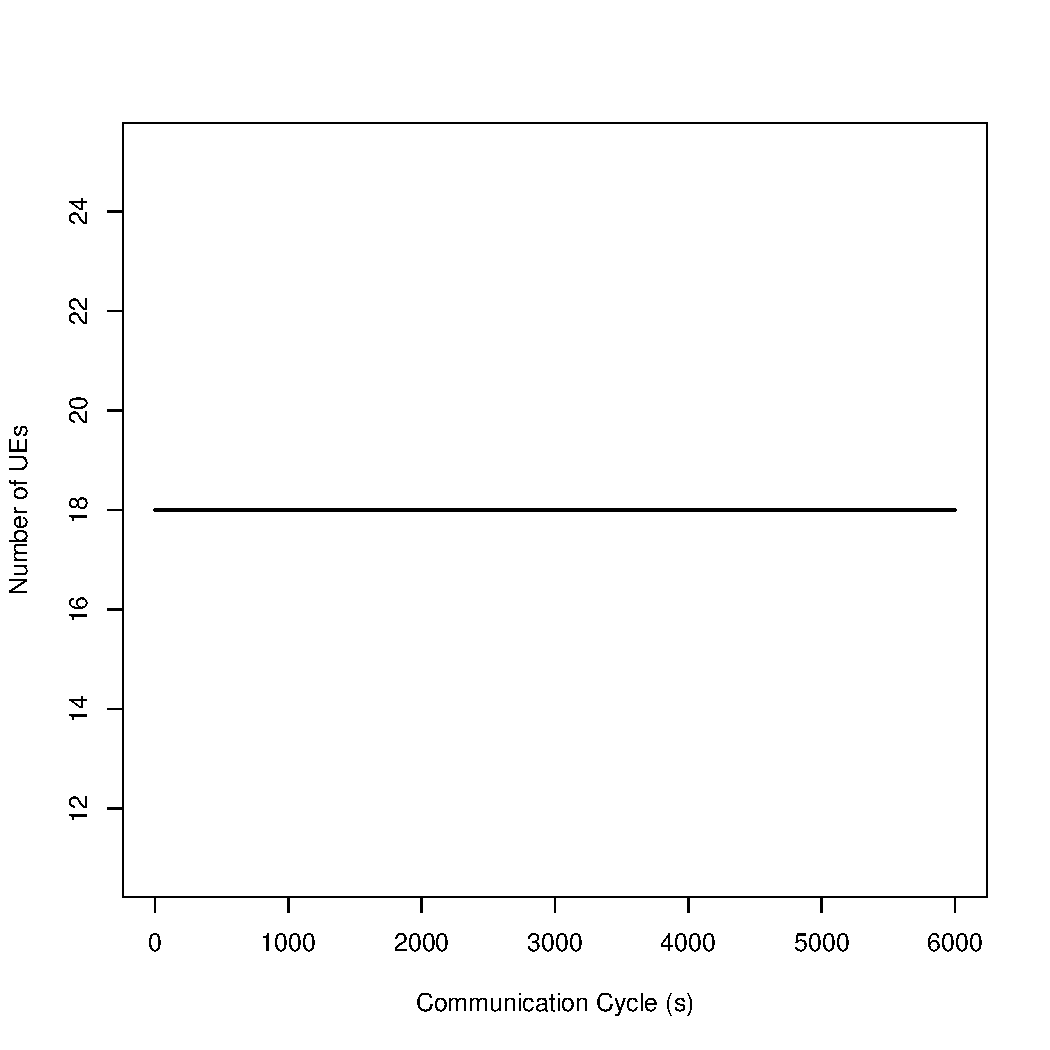
\includegraphics[width=70mm]{UE_cycle_dataset4.pdf}
  \end{center}
  \caption{UE台数と通信周期(データセット4)}
  \label{UE_cycle_dataset4}
 \end{minipage}
 \begin{minipage}{0.5\hsize}
 \begin{center}
  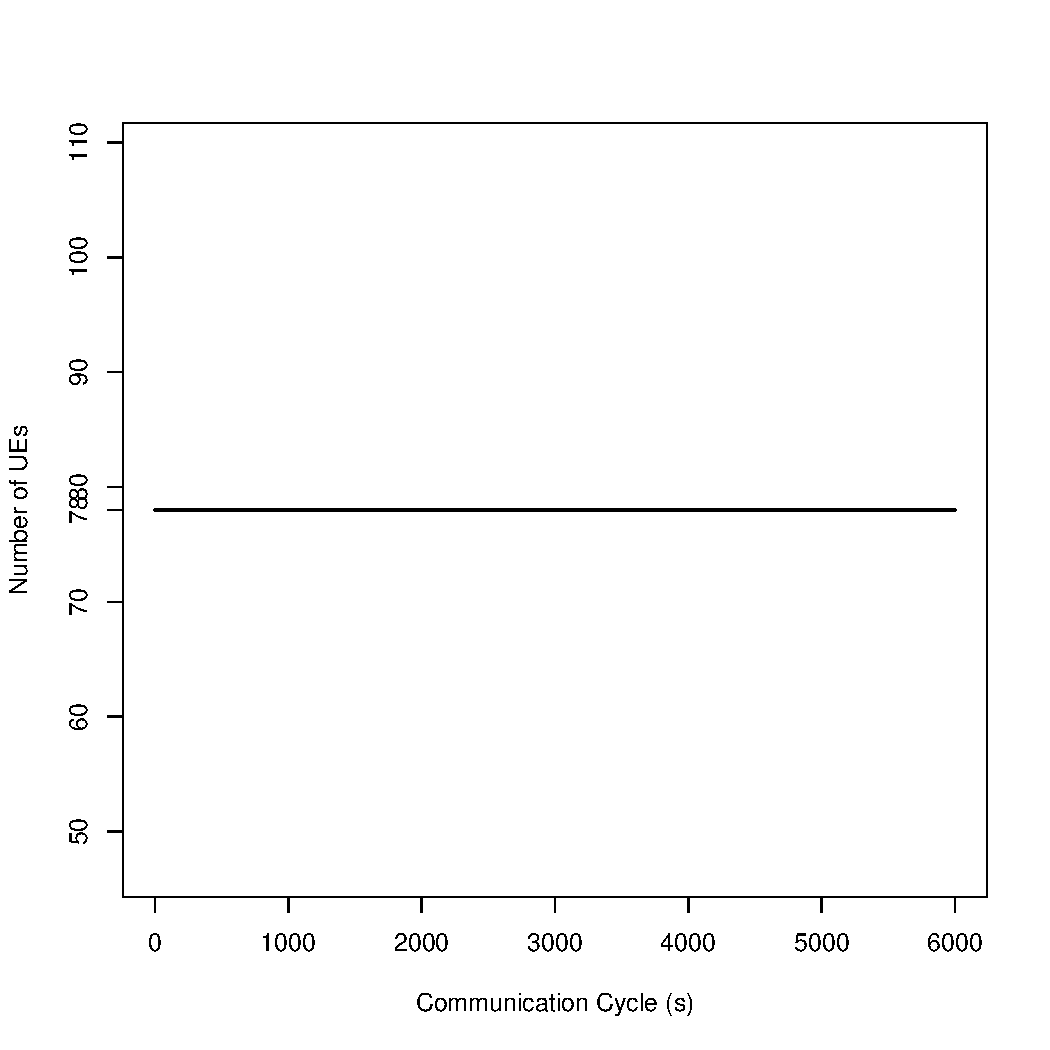
\includegraphics[width=70mm]{UE_cycle_dataset5.pdf}
 \end{center}
  \caption{UE台数と通信周期(データセット5)}
  \label{UE_cycle_dataset5}
 \end{minipage}
 \begin{minipage}{0.5\hsize}
 \begin{center}
  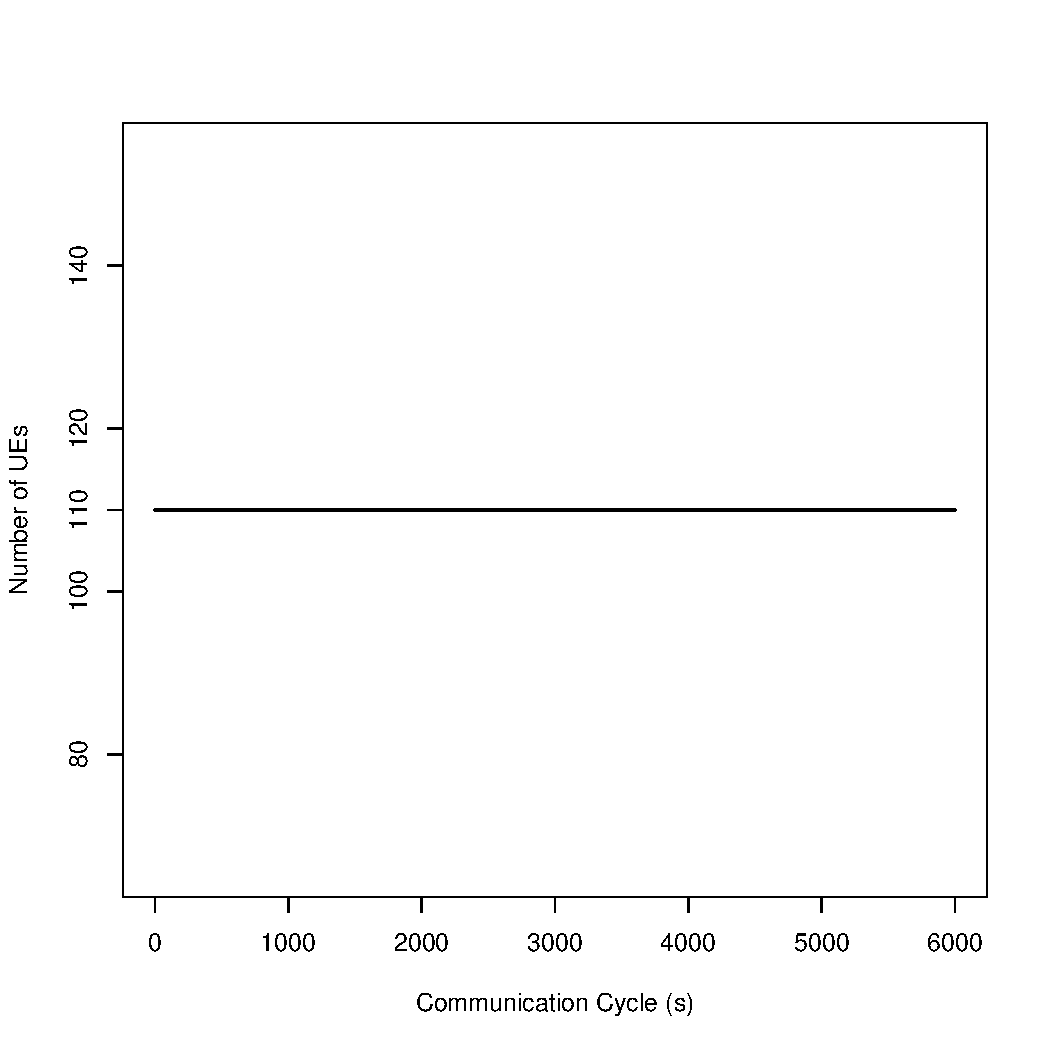
\includegraphics[width=70mm]{UE_cycle_dataset6.pdf}
 \end{center}
  \caption{UE台数と通信周期(データセット6)}
  \label{UE_cycle_dataset6}
 \end{minipage}
\end{figure}

% \begin{figure}[htbp]
%   \centering
%   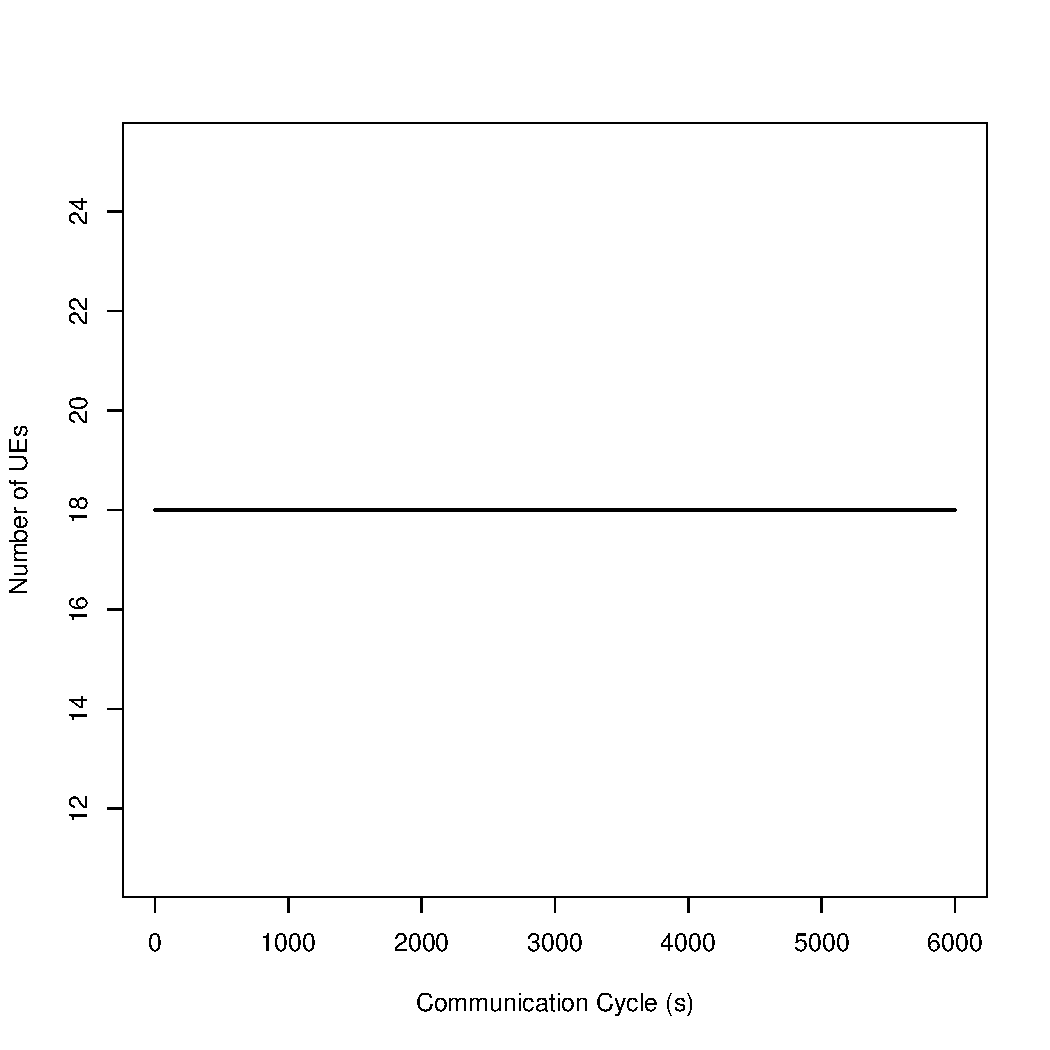
\includegraphics[width=0.5\hsize]{UE_cycle_dataset4.pdf}
%   \caption{通信周期に対するUE台数の分布(データセット4)}
%   \label{UE_cycle_dataset4}
% \end{figure}
%
% \begin{figure}[htbp]
%   \centering
%   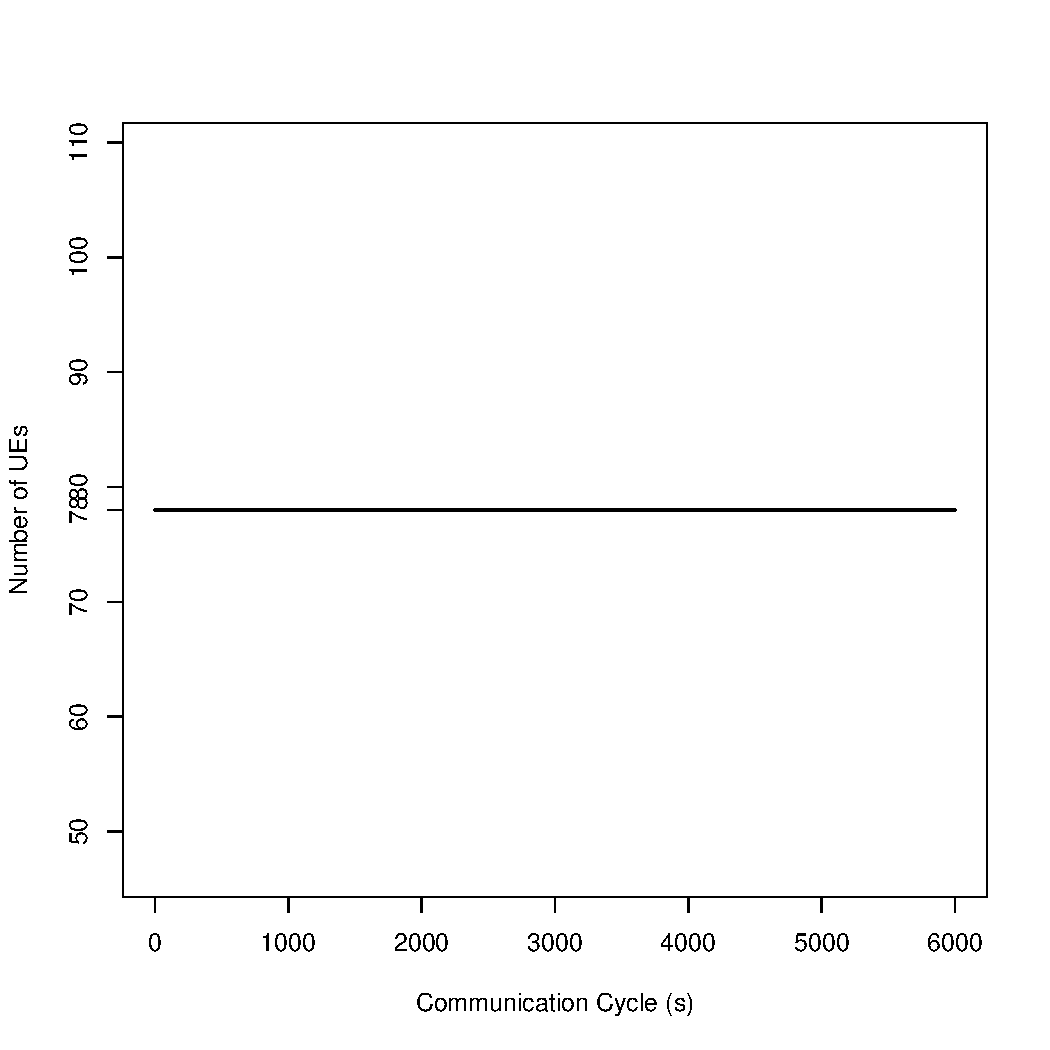
\includegraphics[width=0.5\hsize]{UE_cycle_dataset5.pdf}
%   \caption{通信周期に対するUE台数の分布(データセット5)}
%   \label{UE_cycle_dataset5}
% \end{figure}
%
% \begin{figure}[htbp]
%   \centering
%   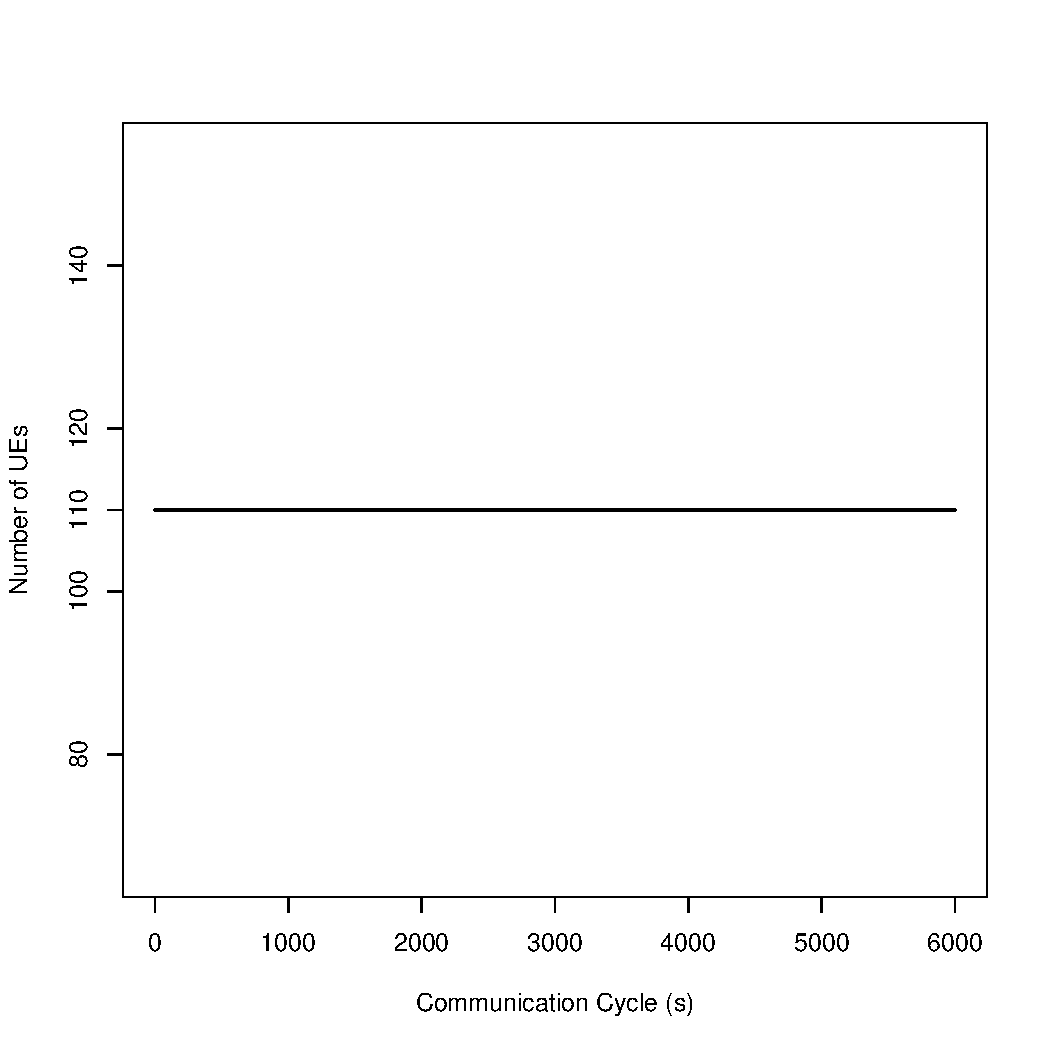
\includegraphics[width=0.5\hsize]{UE_cycle_dataset6.pdf}
%   \caption{通信周期に対するUE台数の分布(データセット6)}
%   \label{UE_cycle_dataset6}
% \end{figure}


% MMEのCPU負荷とMMEのメモリ負荷の関係を示した図を図\ref{4_5_6_signaling_vs_memoryload}に示す。
% また、この図の全体像を図\ref{4_5_6_signaling_vs_memoryload_all}に示す。

MMEのCPU負荷とMMEのメモリ負荷の関係を示した図を図\ref{4_5_6_signaling_vs_memoryload_all}に示す。
データセット4は、$T^{\rm i}$を最小値に設定した場合でも、シグナリング発生数がMMEが処理可能な限界値(1200回/s)を超えないようなUE台数の分布である。
データセット5は、$T^{\rm i}$を最大値に設定した場合でも、メモリ消費量がMMEの限界値(1000MB)を超えないようなUE台数の分布である。
データセット6は、$T^{\rm i}$を適切に設定した場合において、シグナリング発生数およびメモリ消費量がMMEの限界値を超えないようなUE台数の分布である。



これらの結果を見ると、第\ref{sec:estimate1}節で示した結果と比較して、メモリ負荷に対するCPU負荷の制約が相対的に緩くなっている。
これは、通信周期が長いUEの方が、単位時間あたりに発生するシグナリングが少ないという性質が関係している。
本節の評価では、第\ref{sec:estimate1}節と比較して通信周期の長いUEが相対的に多く、通信周期の短いUEが相対的に少ないデータセットを用意したため、ネットワーク全体で見た時のCPU負荷が小さくなっている。
そのため、Idle Timerを変化させCPU負荷とメモリ負荷を相互にオフロードすることにより収容可能なUE台数を向上させる効果が、第\ref{sec:estimate1}節で示した結果と比較して大きい。
実際、Idle Timerを最小に設定した場合(データセット4)とIdle Timerを最大に設定した場合(データセット5)と比較して、収容可能なUE台数はそれぞれ611\%、141\%に向上している。
また、第\ref{sec:estimate1}節で述べた結果と同様に、x軸方向、y軸方向共に、UEの台数と比例の関係があり、グラフの形状は相似である。

% \begin{figure}[htbp]
%   \centering
%   \includegraphics[width=0.9\hsize]{4_5_6_signaling_vs_memoryload.pdf}
%   \caption{MMEに対して発生する、1sあたりのシグナリング数に対するMMEのメモリ負荷(データセット4,5,6)}
%   \label{4_5_6_signaling_vs_memoryload}
% \end{figure}

\begin{figure}[htbp]
  \centering
  \includegraphics[width=0.9\hsize]{4_5_6_signaling_vs_memoryload_all_10s.pdf}
  \caption{MMEに対して発生する、1sあたりのシグナリング数に対するMMEのメモリ負荷の全体像(データセット4,5,6)}
  \label{4_5_6_signaling_vs_memoryload_all}
\end{figure}

\clearpage
%
% \subsection{UEの試算~4}
% \label{sec:estimate4}
% 以下のように条件やパラメータを仮定した。
% \begin{itemize}
%   \item UEごとに通信周期は固定であり、途中で変化することはない。
%   \item 最後の送信が終了したあと、Connected状態のUEがConnected Inactive状態へ遷移するまでの時間($T^{\rm ci}$)は全UEで共通かつ不変の値として$T^{\rm ci} = 10s$とした。
%   \item UEの送信するデータサイズは十分大きいものとする。つまり、データ送信を行うタイミングで必ずConnected状態に遷移するものとする($d_h = 1$)。
%   \item UEの通信周期に対するUE台数の分布は以下の図\ref{UE_cycle_dataset07}、図\ref{UE_cycle_dataset08}、図\ref{UE_cycle_dataset09}に示す、3つのデータセットを用意した。それぞれ、ネットワークに存在するUEの台数は108,000台である。また、通信周期に対してUEの台数は一様分布である。データセット7では1sから3000sの範囲の通信周期のUEが一様分布している。データセット8では、1sから6000sの範囲の通信周期のUEが一様分布している。データセット9では、1sから9000sの範囲の通信周期のUEが一様分布している。
%   \item データ送信にかかる時間はUEの通信周期と比べて十分小さいものとし、送信が失敗することはないと仮定する。
% \end{itemize}
%
% \begin{figure}[htbp]
%  \begin{minipage}{0.5\hsize}
%   \begin{center}
%    \includegraphics[width=70mm]{UE_cycle_dataset07.pdf}
%   \end{center}
%   \caption{UE台数と通信周期(データセット7)}
%   \label{UE_cycle_dataset07}
%  \end{minipage}
%  \begin{minipage}{0.5\hsize}
%  \begin{center}
%   \includegraphics[width=70mm]{UE_cycle_dataset08.pdf}
%  \end{center}
%   \caption{UE台数と通信周期(データセット8)}
%   \label{UE_cycle_dataset08}
%  \end{minipage}
%  \begin{minipage}{0.5\hsize}
%  \begin{center}
%   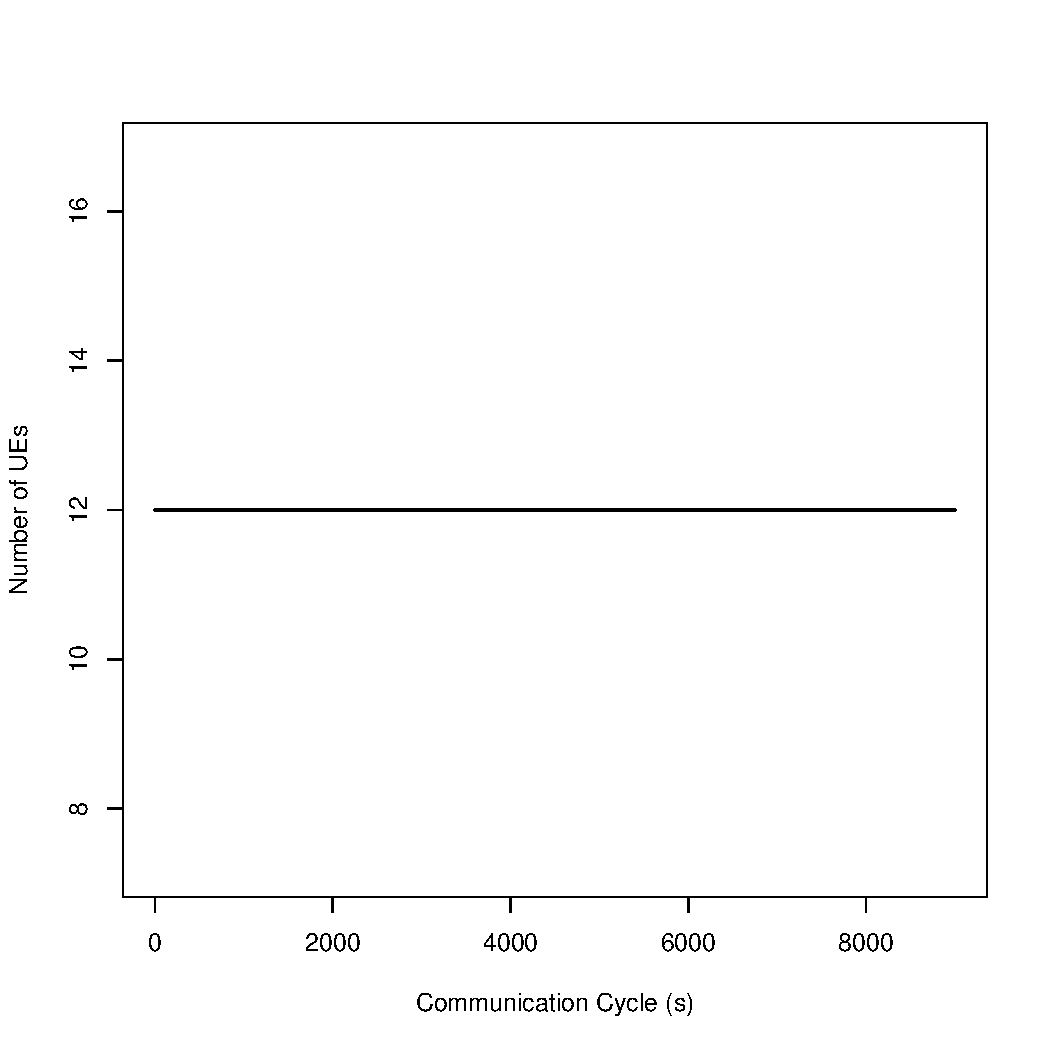
\includegraphics[width=70mm]{UE_cycle_dataset09.pdf}
%  \end{center}
%   \caption{UE台数と通信周期(データセット9)}
%   \label{UE_cycle_dataset09}
%  \end{minipage}
% \end{figure}
%
%
% % \begin{figure}[htbp]
% %   \centering
% %   \includegraphics[width=0.5\hsize]{UE_cycle_dataset07.pdf}
% %   \caption{通信周期に対するUE台数の分布(データセット7)}
% %   \label{UE_cycle_dataset07}
% % \end{figure}
% %
% % \begin{figure}[htbp]
% %   \centering
% %   \includegraphics[width=0.5\hsize]{UE_cycle_dataset08.pdf}
% %   \caption{通信周期に対するUE台数の分布(データセット8)}
% %   \label{UE_cycle_dataset08}
% % \end{figure}
% %
% % \begin{figure}[htbp]
% %   \centering
% %   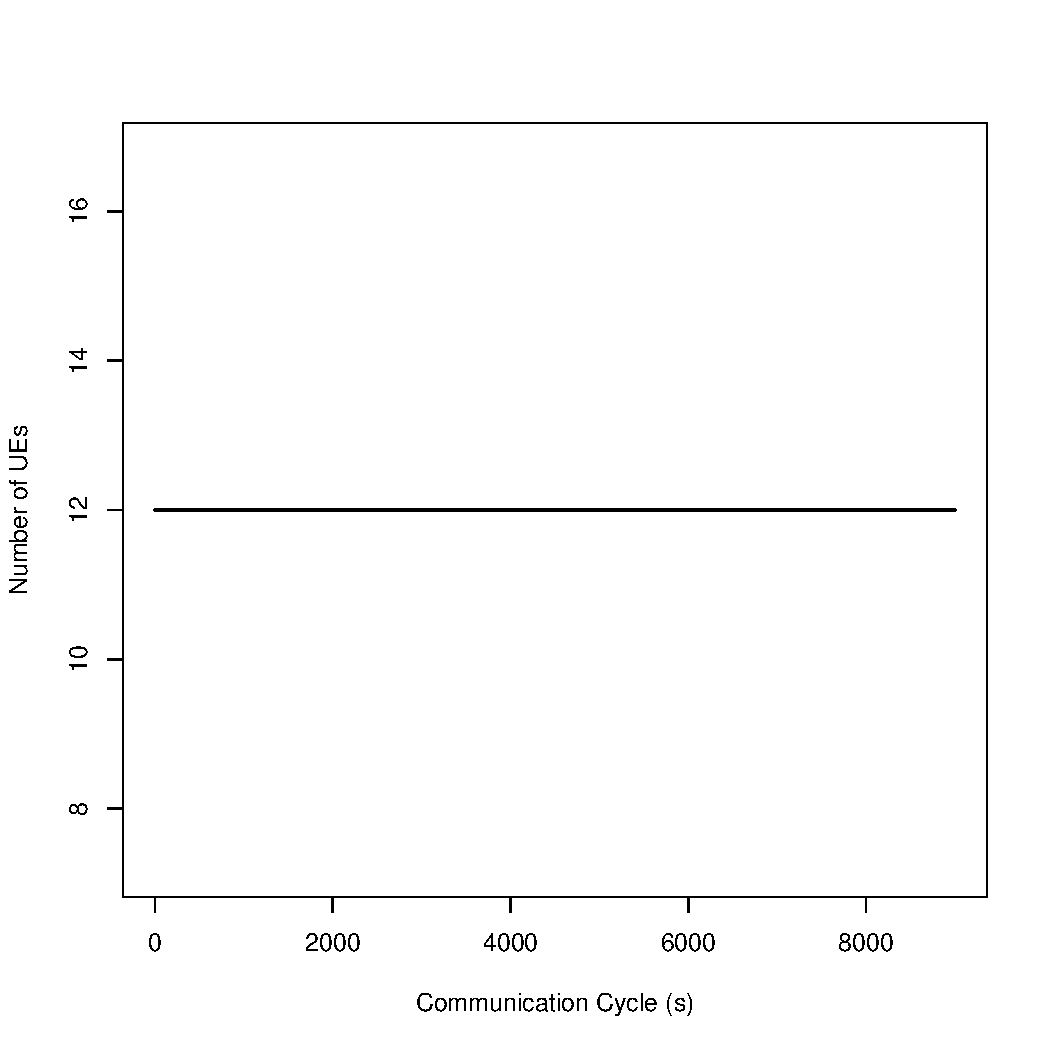
\includegraphics[width=0.5\hsize]{UE_cycle_dataset09.pdf}
% %   \caption{通信周期に対するUE台数の分布(データセット9)}
% %   \label{UE_cycle_dataset09}
% % \end{figure}
%
% \clearpage
%
% 図\ref{7_8_9_signaling_vs_memoryload}に結果を示す。
% まず、y軸切片に着目すると、データセット7、8、9共に同じ値になっていることが分かる。
% このことから、y軸切片はUEの分布に依存しないことが分かる。
% 第\ref{sec:estimate1}節で得られた知見も合わせると、y軸切片はネットワークに存在するUEの台数にのみ比例することが分かる。
%
% 次に、x軸切片付近(Idle Timerを最小に設定してメモリ負荷を出来るだけCPU負荷にオフロードした場合)のCPU負荷に着目する。
% データセット7、8、9のこの値はそれぞれ、2015.7/s、1142.6/s、810.4/sである。
% つまり、UEの通信周期が広い範囲に分布しているデータセットの方がこの値が小さくなることが分かる。
% これは、通信周期が長いUEの方が、単位時間あたりに発生するシグナリングが少ないことが原因である。
% つまり、データセット9の方がデータセット7よりも通信周期の長いUEが相対的に多く、通信周期の短いUEが相対的に少ないため、ネットワーク全体で見た時のCPU負荷が小さくなっている。
%
% UEの分布と、Idle Timer($T^{\rm i}$)を最小に設定した時のCPU負荷($C^{T^{\rm i} = T^{\rm ci}}$)の関係は以下の式(\ref{eq:signaling_max})ように求めることができる。
%
% \begin{eqnarray}
%   $C^{T^{\rm i} = T^{\rm ci}} &=& \int_{k = 1}^{T^{\rm ci}} \frac{1}{k} \cdot (s_{\rm MME}^{\rm ci \to \rm c} + s_{\rm MME}^{\rm c \to \rm ci}) \cdot f(k) dk
%   \\ &+& \int_{k = T^{\rm ci}}^{\infty} \frac{1}{k} \cdot (s_{\rm MME}^{\rm i \to \rm c} + s_{\rm MME}^{\rm c \to \rm ci} + s_{\rm MME}^{\rm ci \to \rm i}) \cdot f(k)  dk $
%    \label{eq:signaling_max}
% \end{eqnarray}
%
% ここで、$f$は通信周期に対するUEの分布を表す関数とする。
% 例えば、$f(3)$とすると、通信周期が3sのUEの台数を表す。
%
% ここで、今回の評価のように、UEの通信周期の分布が最大値を$w(s)$とするような一様分布で表現できる場合は、以下の式(\ref{eq:signaling_max_2})のように式を書き換えることができる。
% \begin{eqnarray}
%   $C^{T^{\rm i} = T^{\rm ci}}  &=&  \int_{k = 1}^{T^{\rm ci}} \frac{1}{k} \cdot (s_{\rm MME}^{\rm ci \to \rm c} + s_{\rm MME}^{\rm c \to \rm ci}) \cdot \frac{N_{\rm UE}}{w}  dk
%    \\ &+& \int_{k = T^{\rm ci}}^{w} \frac{1}{k} \cdot (s_{\rm MME}^{\rm i \to \rm c} + s_{\rm MME}^{\rm c \to \rm ci} + s_{\rm MME}^{\rm ci \to \rm i}) \cdot \frac{N_{\rm UE}}{w}  dk $
%   \label{eq:signaling_max_2}
% \end{eqnarray}
%
% さらに、今回の評価の場合は$s_{\rm MME}^{\rm ci \to \rm c} + s_{\rm MME}^{\rm c \to \rm ci}$が0であることを考慮して、以下のように式を簡略化できる。
% \begin{eqnarray}
%   $C^{T^{\rm i} = T^{\rm ci}} & = & (s_{\rm MME}^{\rm i \to \rm c} + s_{\rm MME}^{\rm c \to \rm ci} + s_{\rm MME}^{\rm ci \to \rm i})  \cdot \frac{N_{\rm UE}}{w} \cdot \int_{k = T^{\rm ci}}^{w} \frac{1}{k}   dk $ \label{eq:signaling_max_3}
% \end{eqnarray}
% 自明ではないが、$\frac{1}{w} \cdot \int_{k = T^{\rm ci}}^{w} \frac{1}{k} $は$w$に関して単調減少である。
% 以上の理由で、通信周期の分布の幅が広い方が、CPU負荷が小さくなる。
% \begin{figure}[htbp]
%   \centering
%   \includegraphics[width=0.9\hsize]{7_8_9_signaling_vs_memoryload_100s.pdf}
%   \caption{MMEに対して発生する、1sあたりのシグナリング数に対するMMEのメモリ負荷(データセット7,8,9)}
%   \label{7_8_9_signaling_vs_memoryload}
% \end{figure}

\clearpage
\subsection{UEの試算~4}
\label{sec:estimate4}
3GPPの仕様書\cite{3gpp.45.820}を参考にし、以下のように条件やパラメータを仮定した。
\begin{itemize}
  \item UEごとに通信周期は固定であり、途中で変化することはない。
  \item 最後の送信が終了したあと、Connected状態のUEがConnected Inactive状態へ遷移するまでの時間($T^{\rm ci}$)は全UEで共通かつ不変の値として$T^{\rm ci} = 10s$とした。
  \item UEの送信するデータサイズは十分大きいものとする。つまり、データ送信を行うタイミングで必ずConnected状態に遷移するものとする($d_h = 1$)。
  \item UEの通信周期に対するUE台数の分布を以下の図\ref{UE_cycle_dataset10}、図\ref{UE_cycle_dataset11}、図\ref{UE_cycle_dataset12}に示す。ネットワークに存在するUEの台数はそれぞれ、925,700、469,200、1,178,100台である。
  \item データ送信にかかる時間はUEの通信周期と比べて十分小さいものとし、送信が失敗することはないと仮定する。
\end{itemize}

\begin{figure}[htbp]
 \begin{minipage}{0.5\hsize}
  \begin{center}
   \includegraphics[width=70mm]{UE_cycle_dataset10.pdf}
  \end{center}
  \caption{UE台数と通信周期(データセット10)}
  \label{UE_cycle_dataset10}
 \end{minipage}
 \begin{minipage}{0.5\hsize}
 \begin{center}
  \includegraphics[width=70mm]{UE_cycle_dataset11.pdf}
 \end{center}
  \caption{UE台数と通信周期(データセット11)}
  \label{UE_cycle_dataset11}
 \end{minipage}
 \begin{minipage}{0.5\hsize}
 \begin{center}
  \includegraphics[width=70mm]{UE_cycle_dataset12.pdf}
 \end{center}
  \caption{UE台数と通信周期(データセット12)}
  \label{UE_cycle_dataset12}
 \end{minipage}
\end{figure}

結果を図\ref{10_11_12_signaling_vs_memoryload}に示す。
データセット10は、$T^{\rm i}$を最小値に設定した場合でも、シグナリング発生数がMMEが処理可能な限界値(1200回/s)を超えないようなUE台数の分布である。
データセット11は、$T^{\rm i}$を最大値に設定した場合でも、メモリ消費量がMMEの限界値(1000MB)を超えないようなUE台数の分布である。
データセット12は、$T^{\rm i}$を適切に設定した場合において、シグナリング発生数およびメモリ消費量がMMEの限界値を超えないようなUE台数の分布である。
この結果より、Idle Timerを適切に設定した場合は、Idle Timerを最小に設定した場合と最大に設定した場合それぞれと比較して、収容可能なUE台数が127\%および251\%に増加したことが分かる。
\begin{figure}[htbp]
  \centering
  \includegraphics[width=0.9\hsize]{10_11_12_signaling_vs_memoryload_all_300s.pdf}
  \caption{MMEに対して発生する、1sあたりのシグナリング数に対するMMEのメモリ負荷(データセット10,11,12)}
  \label{10_11_12_signaling_vs_memoryload}
\end{figure}

\clearpage


% Idle Timer($T^{\rm i}$)をある値$\alpha (\alpha \ge T^{\rm ci})$に設定した時のCPU負荷は、式(\ref{eq:attach_detach})および(\ref{eq:all_signal})の$T^{\rm i}$に$\alpha$を代入することによって求められる以下の式(\ref{eq:signaling_load_all_UE})、(\ref{eq:signaling_load})より得られる。
% 式(\ref{eq:attach_detach})および(\ref{eq:all_signal})の$T^{\rm i}$に$\alpha$を代入した時に導出される$C$を$C(\alpha)$と定義する。


% \begin{eqnarray}
% \begin{split}
%   C(\alpha) &= \int_{k = 0}^{T^{\rm ci}} \frac{1}{k} \cdot s_{\rm MME}^{\rm c \to \rm c} \cdot f(k) \cdot N_{\rm UE} dk
%   \\ &+ \int_{k = T^{\rm ci}}^{\alpha} \frac{1}{k} \cdot (s_{\rm MME}^{\rm ci \to \rm c} + s_{\rm MME}^{\rm c \to \rm ci}) \cdot f(k) \cdot N_{\rm UE} dk
%   \\ &+ \int_{k = \alpha}^{\infty} \frac{1}{k} \cdot (s_{\rm MME}^{\rm i \to \rm c} + s_{\rm MME}^{\rm c \to \rm ci} + s_{\rm MME}^{\rm ci \to \rm i}) \cdot f(k) \cdot N_{\rm UE} dk
%    \label{eq:signaling_load}
% \end{split}
% \end{eqnarray}

% \begin{eqnarray}
% \begin{split}
%   C(\alpha) &= \sum_{h = 1}^{N_{\rm UE}} c_h(\alpha) \label{eq:signaling_load_all_UE}
% \end{split}
% \end{eqnarray}
%
% \begin{equation}
%   c_h(\alpha)  =
%   \begin{cases}
% 		\frac{1}{T_h} \cdot s_{\rm MME}^{\rm c \to \rm c} & \text{if $T_h \le T^{\rm ci}$} \\
%     \frac{1}{T_h} \cdot (s_{\rm MME}^{\rm ci \to \rm c} + s_{\rm MME}^{\rm c \to \rm ci}) \cdot d_h  + \frac{1}{T_h} \cdot s_{\rm MME}^{\rm ci \to \rm ci} \cdot (1 - d_h) & \text{if $T^{\rm ci} < T_h \le \alpha $} \\
%     \frac{1}{T_h} \cdot (s_{\rm MME}^{\rm i \to \rm c} + s_{\rm MME}^{\rm c \to \rm ci} + s_{\rm MME}^{\rm ci \to \rm i}) & \text{otherwise}
%   \end{cases}
%   \label{eq:signaling_load}
% \end{equation}

% ここで、$N_{\rm UE}$は全UEの台数、$f$はUEの通信周期の確率密度関数とする。
% 例えば、$\int_3^4 f(k) \cdot N_{\rm UE} dk$とすると、通信周期が3s以上 〜 4s以下 のUEの台数を表す。
% また、今回の評価の場合は$s_{\rm MME}^{\rm c \to \rm c} = 0$および$s_{\rm MME}^{\rm ci \to \rm c} + s_{\rm MME}^{\rm c \to \rm ci} = 0$であることを考慮して、以下の式(\ref{eq:signaling_load_simple})のように簡略化できる。
%
% \begin{eqnarray}
%   C(\alpha) = \int_{k = \alpha}^{\infty} \frac{1}{k} \cdot (s_{\rm MME}^{\rm i \to \rm c} + s_{\rm MME}^{\rm c \to \rm ci} + s_{\rm MME}^{\rm ci \to \rm i}) \cdot f(k) \cdot N_{\rm UE}  dk
%   \label{eq:signaling_load_simple}
% \end{eqnarray}

% 次に、Idle Timer($T^{\rm i}$)をある値$\alpha (\alpha \ge T^{\rm ci})$に設定した時のメモリ負荷は式(\ref{eq:connected})、(\ref{eq:inactive})、(\ref{eq:idle})、(\ref{eq:MME_memory})および(\ref{eq:all_memory})の$T^{\rm i}$に$\alpha$を代入することによって求められる以下の式(\ref{eq:memory_load_all_UE})、(\ref{eq:memory_load})、(\ref{eq:connected_alpha})、(\ref{eq:inactive_alpha})および(\ref{eq:idle_alpha})より得られる。
% これらの式の$T^{\rm i}$に$\alpha$を代入した時に導出される$M$を$M(\alpha)$と定義する。

% \begin{eqnarray}
%   M(\alpha) & = & \sum_{h = 1}^{N_{\rm UE}} m_h(\alpha) \label{eq:memory_load_all_UE}
% \end{eqnarray}
%
% \begin{eqnarray}
%   m_h(\alpha) & = & m^{\rm c}_{\rm MME} \cdot \tau^{\rm c}_h(\alpha) + m^{\rm ci}_{\rm MME} \cdot \tau^{\rm ci}_h(\alpha) + m^{\rm i}_{\rm MME} \cdot \tau^{\rm i}_h(\alpha) \label{eq:memory_load}
% \end{eqnarray}
%
% \begin{align}
% 	\tau^{\rm c}_h(\alpha) & =
% 	\begin{cases}
%     1 \hphantom{100000000000000} & \text{if $T_h \le T^{\rm ci}$}\\
%     \frac{T^{\rm ci}}{T_h} \cdot d_h + \frac{0}{T_h} \cdot (1 - d_h)& \text{if $T^{\rm ci} < T_h \le \alpha$}\\
%     \frac{T^{\rm ci}}{T_h} & \text{otherwise}
%   \end{cases} \label{eq:connected_alpha}\\
% 	\tau^{\rm ci}_h(\alpha) & =
%   \begin{cases}
%     0 \hphantom{100000000000000} & \text{if $T_h \le T^{\rm ci}$}\\
% 		\frac{T_h - T^{\rm ci}}{T_h} \cdot d_h + \frac{T_h}{T_h} \cdot (1 - d_h) & \text{if $T^{\rm ci} < T_h \le \alpha$}\\
%     \frac{\alpha - T^{\rm ci}}{T_h} & \text{otherwise}
%   \end{cases} \label{eq:inactive_alpha}\\
% 	\tau^{\rm i}_h(\alpha) & =
%   \begin{cases}
%     0 \hphantom{100000000000000} & \text{if $T_h \le T^{\rm ci}$}\\
% 		0 & \text{if $T^{\rm ci} < T_h \le \alpha$}\\
%     \frac{T_h - \alpha}{T_h} & \text{otherwise}
%   \end{cases}\label{eq:idle_alpha}
% \end{align}

% \begin{eqnarray}
% \begin{split}
%   M(\alpha) &= \int_{k = 0}^{T^{\rm ci}} m^{\rm c}_{\rm MME} \cdot f(k) \cdot N_{\rm UE} dk
%   \\ &+ \int_{k = T^{\rm ci}}^{\alpha} \frac{1}{k} \cdot (T^{\rm ci} \cdot m^{\rm c}_{\rm MME} + (k - T^{\rm ci}) \cdot m^{\rm ci}_{\rm MME}) \cdot f(k) \cdot N_{\rm UE}  dk
%   \\ &+ \int_{k = \alpha}^{\infty} \frac{1}{k} \cdot (T^{\rm ci} \cdot m^{\rm c}_{\rm MME} + (\alpha - T^{\rm ci}) \cdot m^{\rm ci}_{\rm MME} + (k - \alpha) \cdot m^{\rm i}_{\rm MME}) \cdot f(k) \cdot N_{\rm UE}  dk
%   \label{eq:memory_load}
% \end{split}
% \end{eqnarray}

% 今回の評価の場合は$m_{\rm MME}^{\rm c} = m_{\rm MME}^{\rm ci}$であることを考慮して、以下の式(\ref{eq:memory_load_simple})のように簡略化できる。
% \begin{eqnarray}
% \begin{split}
%   M(\alpha) &= \int_{k = 0}^{\alpha} m^{\rm ci}_{\rm MME} \cdot f(k) \cdot N_{\rm UE} dk
%   % \\ &+ \int_{k = T^{\rm ci}}^{\alpha} \frac{1}{k} \cdot (T^{\rm ci} \cdot m^{\rm c}_{\rm MME} + (k - T^{\rm ci}) \cdot m^{\rm ci}_{\rm MME}) \cdot f(k)  dk
%   \\ &+ \int_{k = \alpha}^{\infty} \frac{1}{k} \cdot (\alpha \cdot m^{\rm ci}_{\rm MME} + (k - \alpha) \cdot m^{\rm i}_{\rm MME}) \cdot f(k) \cdot N_{\rm UE}  dk
%   \label{eq:memory_load_simple}
% \end{split}
% \end{eqnarray}



% ここで、今回の評価のように、UEの通信周期の分布が最大値を$w(s)$とするような一様分布で表現できる場合は、以下の式(\ref{eq:signaling_max_2})のように式を書き換えることができる。
% \begin{eqnarray}
%   $C^{T^{\rm i} = T^{\rm ci}}  &=&  \int_{k = 1}^{T^{\rm ci}} \frac{1}{k} \cdot (s_{\rm MME}^{\rm ci \to \rm c} + s_{\rm MME}^{\rm c \to \rm ci}) \cdot \frac{N_{\rm UE}}{w}  dk
%    \\ &+& \int_{k = T^{\rm ci}}^{w} \frac{1}{k} \cdot (s_{\rm MME}^{\rm i \to \rm c} + s_{\rm MME}^{\rm c \to \rm ci} + s_{\rm MME}^{\rm ci \to \rm i}) \cdot \frac{N_{\rm UE}}{w}  dk $
%   \label{eq:signaling_max_2}
% \end{eqnarray}
%
% さらに、今回の評価の場合は$s_{\rm MME}^{\rm ci \to \rm c} + s_{\rm MME}^{\rm c \to \rm ci}$が0であることを考慮して、以下のように式を簡略化できる。
% \begin{eqnarray}
%   $C^{T^{\rm i} = T^{\rm ci}} & = & (s_{\rm MME}^{\rm i \to \rm c} + s_{\rm MME}^{\rm c \to \rm ci} + s_{\rm MME}^{\rm ci \to \rm i})  \cdot \frac{N_{\rm UE}}{w} \cdot \int_{k = T^{\rm ci}}^{w} \frac{1}{k}   dk $ \label{eq:signaling_max_3}
% \end{eqnarray}
% 自明ではないが、$\frac{1}{w} \cdot \int_{k = T^{\rm ci}}^{w} \frac{1}{k} $は$w$に関して単調減少である。
% 以上の理由で、通信周期の分布の幅が広い方が、CPU負荷が小さくなる。
\subsection{UEの試算~5}
\label{sec:estimate5}
文献\cite{Machine-to-MachineCommunicationsArchitecturesTechnologyStandardsandApplications}を参考にし、以下のように条件やパラメータを仮定した。
\begin{itemize}
  \item UEごとに通信周期は固定であり、途中で変化することはない。
  \item 最後の送信が終了したあと、Connected状態のUEがConnected Inactive状態へ遷移するまでの時間($T^{\rm ci}$)は全UEで共通かつ不変の値として$T^{\rm ci} = 10s$とした。
  \item UEの送信するデータサイズは十分大きいものとする。つまり、データ送信を行うタイミングで必ずConnected状態に遷移するものとする($d_h = 1$)。
  \item UEの通信周期に対するUE台数の分布を以下表\ref{table:CityCommercialM2MDevice}示す。ネットワークに存在するUEの台数はそれぞれ、469,200、24,192、480,619台である。
  \item データ送信にかかる時間はUEの通信周期と比べて十分小さいものとし、送信が失敗することはないと仮定する。
\end{itemize}

\begin{table}[h]
 \caption{City Commercial M2M Device}
 \label{table:CityCommercialM2MDevice}
 \centering
  \begin{tabular}{ccc}
   \hline
   Device & Average Message & Number of Device Ratio\\
   & Transmission Rate/s & (New York City) \\
   \hline \hline
    credit machine in grocery & 120s & 7.41\%  \\
    credit machine in shop & 1800s & 77.85\% \\
    Roadway signs & 30s & 11.20\%  \\
    Traffic lights & 60s & 0.53\%  \\
    Traffic sensor & 60s & 0.53\%  \\
    Movie rental machine & 86400s & 2.47\%  \\
   \hline
  \end{tabular}
\end{table}
% \begin{table}[h]
%  \caption{City Commercial M2M Device}
%  \label{table:CityCommercialM2MDevice}
%  \centering
%   \begin{tabular}{cccc}
%    \hline
%    Device & Average Message & \multicolumn{2}{c}{Number of Device Ratio(\%)} \\
%    & Transmission Rate/s & Urban & Suburban \\
%    \hline \hline
%     credit machine in grocery & 120s & 7.41\% & 1.49\%  \\
%     credit machine in shop & 1800s & 77.85\% & 22.48\%  \\
%     Roadway signs & 30s & 11.20\% & 60.59\%  \\
%     Traffic lights & 60s & 0.53\% & 7.35\%  \\
%     Traffic sensor & 60s & 0.53\% & 7.35\%  \\
%     Movie rental machine & 86400s & 2.47\% & 0.74\%  \\
%    \hline
%   \end{tabular}
% \end{table}

% device urban(New York City) Suburban(Washington DC)
% credit machine in grocery 120s  7.41% 1.49%
% credit machine in shop 1800s  77.85%  22.48%
% Roadway signs 30s 11.20%  60.59%
% Traffic lights 60s  0.53% 7.35%
% Traffic sensor 60s  0.53% 7.35%
% Movie rental machine 86400s 2.47% 0.74%
%
% 0.00020947(7.412716%) 0.0022(77.853508%) 0.00031647(11.199227%) 0.00001503(0.531881%) 0.00001503(0.531881%) 0.000069823(2.47089%) (sum)0.00282582
% 7.41% 77.85% 11.20% 0.53% 0.53% 2.47%
%
% 2.3122(1.49%) 34.988(22.48%) 94.325(60.59%) 11.442(7.35%) 11.442(7.35%) 1.1561(0.74%) (sum)155.6653

結果を図\ref{13_14_15_signaling_vs_memoryload_all_15s}に示す。
データセット13は、$T^{\rm i}$を最大値に設定した場合でも、メモリ消費量がMMEの限界値(1000MB)を超えないようなUE台数(469,200台)の分布である。
データセット14は、$T^{\rm i}$を最小値に設定した場合でも、シグナリング発生数がMMEが処理可能な限界値(1200回/s)を超えないようなUE台数(24,192台)の分布である。
データセット15は、$T^{\rm i}$を適切に設定した場合において、シグナリング発生数およびメモリ消費量がMMEの限界値を超えないようなUE台数(480,619台)の分布である。
この結果より、Idle Timerを適切に設定した場合は、Idle Timerを最小に設定した場合比較して、収容可能なUE台数が19倍に増加したことがわかる。
一方、Idle Timerを最大に設定した場合と比較すると収容可能なUE台数の差は小さく、1.02倍に増加している。
\begin{figure}[htbp]
  \centering
  \includegraphics[width=0.9\hsize]{13_14_15_signaling_vs_memoryload_all_15s.pdf}
  \caption{MMEに対して発生する、1sあたりのシグナリング数に対するMMEのメモリ負荷(データセット13,14,15)}
  \label{13_14_15_signaling_vs_memoryload_all_15s}
\end{figure}

\section{まとめ}
消費電力はあまり変わらないと考えられる。
\begin{description}
  \item[日付] 2009年5月30日
  \item[会場] 居酒屋Snoopy
  \item[予算] 4,500円
\end{description}
\clearpage


  \section{今後の予定}
  \begin{itemize}
    \item IdleTimerの設定方法を決める良いアルゴリズムがないか調査する。
  \end{itemize}

\section*{\addcontentsline{toc}{section}{参考文献}}
\bibliographystyle{IEEEtran}
\bibliography{/Users/t-adachi/Documents/study/Bibliography/bib/hpt_core_network/myBib/LABbiblio,/Users/t-adachi/Documents/study/Bibliography/bib/hpt_core_network/Study_Group_Bibtex/bib/hptCoreNetwork_Study}
\end{document}
